\begin{figure}
  \setlength{\unitlength}{\textwidth}
\fbox{
        \begin{picture}(1,1.1)(0,0.4)

      % % % Parkinson Data 
      \put(0.1,1.1){\includegraphics[width=0.75\unitlength]{../FnP/gnuplot/displacement_low_pi_1.eps}}
      \put(0.1,0.76){\includegraphics[width=0.75\unitlength]{../FnP/gnuplot/velocity_low_pi_1.eps}}
      \put(0.1,0.42){\includegraphics[width=0.75\unitlength]{../FnP/gnuplot/mean_power_low_pi_1.eps}}
      
       \put(0.07,0.95){$\displaystyle\frac{V}{D}$}
       \put(0.07,1.3){$\displaystyle\frac{A}{D}$}
       \put(0.05,0.6){$\displaystyle\frac{P_{m}}{\rho \mathcal{A}U^3 }$}
       \put(0.5,0.4){$\massdamp$}
       \
\put(0.189,1.415){\small(a)}
\put(0.189,1.07){\small(b)}
\put(0.189,0.73){\small(c)}

%  

      
    \end{picture}
}
  \caption{Comparison of QSS data at high and low \ \massstiff. (a) displacement amplitude, (b) velocity amplitude and (c) mean power as a function of \massdamp. Data presented at $\massstiff=100 \ (\times) \ \mstar=130 (+)$, \  $\massstiff=0.1 \ \mstar=2$ (\ding{117}), \  $\massstiff=0.1 \ \mstar=20 \ (\triangle)$ and  $\massstiff=0.1 \ \mstar=50 \ (*)$. The mass ratio does not have an effect on \massstiff even at low \massstiff}
    \label{fig:low_pi_1}
\end{figure}

 %vspace{10cm}
